\documentclass{article}
\usepackage[utf8]{inputenc}
\usepackage[spanish]{babel}
\usepackage{graphicx}
\usepackage{geometry}
\usepackage{enumerate}
\usepackage{titlesec}
\usepackage{float}
\usepackage{amsmath}

\geometry{letterpaper, margin = 1.5cm}

%Datos de la Portada
\title{Herrramientas Computacionales \\ Practica 3. Manejo de Arreglos.}
\author{Medina Martinez Jonathan Jason \\ 2023640061}
\date{14 de marzo de 2023}

\begin{document} %Inicio del Documento

\fontsize{12}{14}\selectfont

\begin{figure}[t] %Logos Portada


\includegraphics[width=2.5 cm]{Logo1.jpeg}
\hfill

\includegraphics[width=3 cm]{Logo2.png}

\end{figure}

\maketitle %Titulo Portada
\newpage

\tableofcontents %Indice
\newpage

\section{Objetivo}

Aplicar la estructura de un arreglo para el manejo de datos

\section{Introducción}

En esta practica se realizaran diversas Matricez a traves de arreglos de datos.

\newpage

\section{Desarrollo}

\subsection{Cree un vector fila en el cual el primer elemento sea 1 y el ultimo sea 33, con una distancia de 2 entre los elementos.}

\begin{figure}[H]
    \centering
    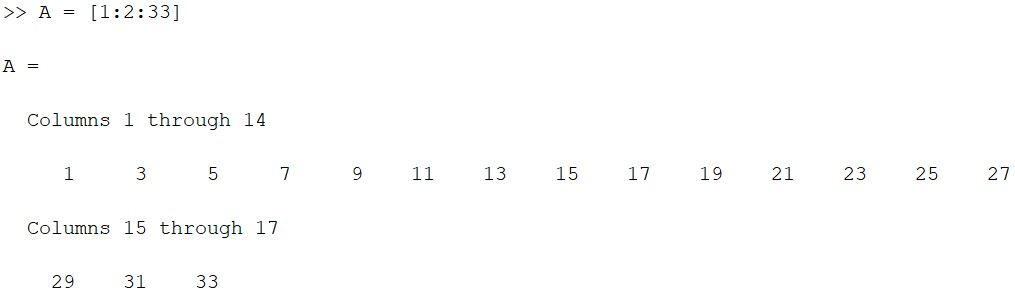
\includegraphics[width = 16cm]{img1.jpg}
\end{figure}

\subsection{Cree un vector columna en el cual el primer elemento sea 15, la distancia de los elementos sea -5, y el  ́Ultimo elemento sea -25.}

\begin{figure}[H]
    \centering
    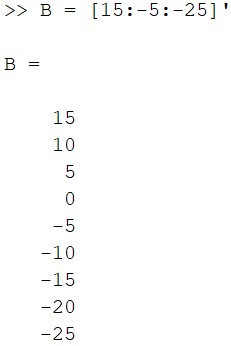
\includegraphics[width = 5cm]{img2.jpg}
\end{figure}

\subsection{Cree un vector fila con 15 elementos igualmente distanciados, en el cual el primer elementos sea 7 y el ultimo 40.}

\begin{figure}[H]
    \centering
    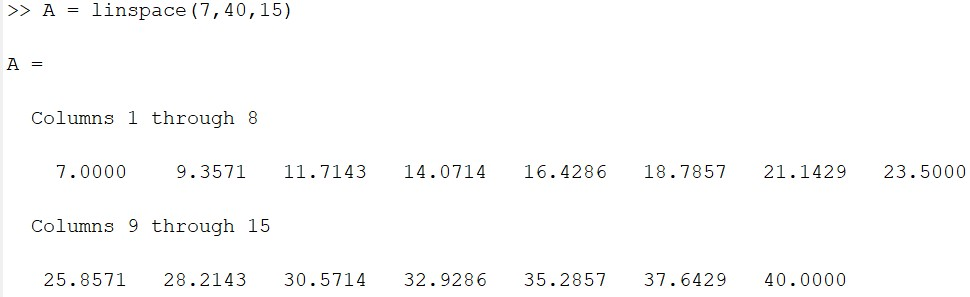
\includegraphics[width = 16cm]{img3.jpg}
\end{figure}

\subsection{Cree un vector columna con 12 elementos igualmente distanciados, en el cual el primer elemento sea -1 y el  ́ultimo -15.}

\begin{figure}[H]
    \centering
    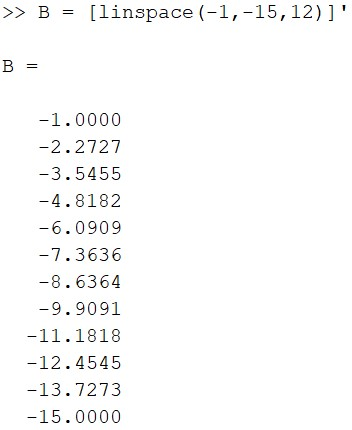
\includegraphics[width = 8cm]{img4.jpg}
\end{figure}

\subsection{Cree un vector llamado Auno, que tenga 16 elementos, siendo el primero el 4, con un incremento de 3 y ultimo elemento 49. Utilizando el simbolo dos puntos (:), cree un nuevo vector llamado Ados que tenga ocho elementos, de tal forma que los primeros cuatro sean los primeros cuatros del vector Auno, y los  ́ultimos cuatro sean los ultimos cuatro del vector Auno.}

\begin{figure}[H]
    \centering
    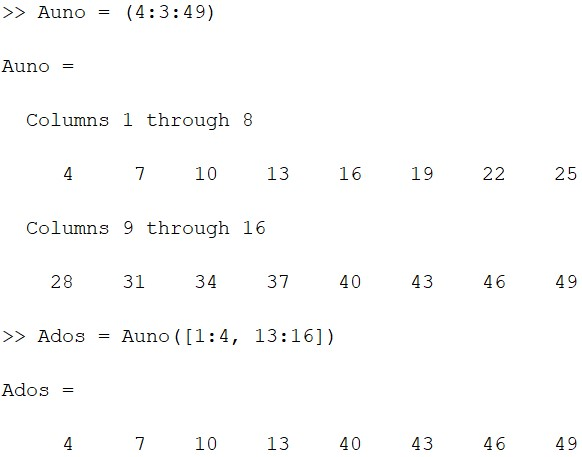
\includegraphics[width = 12cm]{img5.jpg}
\end{figure}

\subsection{Cree la siguiente matriz:}

\begin{equation*}
A =
\begin{pmatrix}
6 & 43 & 2 & 11 & 87 \\
12 & 6 & 34 & 0 & 5 \\
34 & 18 & 7 & 41 & 9
\end{pmatrix}
\end{equation*}
\
\
\
\
\begin{figure}[H]
    \centering
    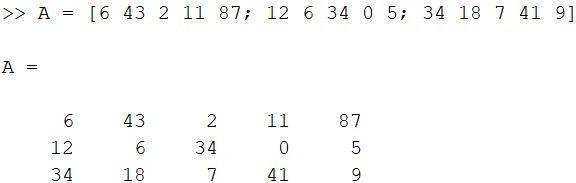
\includegraphics[width = 15cm]{img6.jpg}
\end{figure}
\
\
\
\
Utilice la matriz A para:
\
\
\
\
\subsubsection{Crear un vector fila de cinco elementos llamado va, que contenga los elementos de la segunda fila de A.}
\begin{figure}[H]
    \centering
    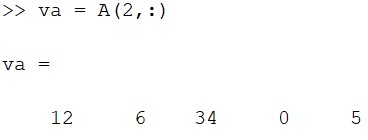
\includegraphics[width = 12cm]{img6a.jpg}
\end{figure}
\subsubsection{Crear un vector fila de seis elementos llamado vb, que contenga los elementos de la cuarta y quinta columna de A.}
\begin{figure}[H]
    \centering
    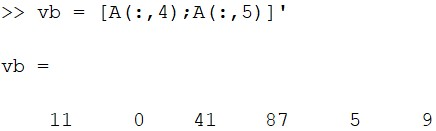
\includegraphics[width = 12cm]{img6b.jpg}
\end{figure}
\subsubsection{Crear un vector fila de diez elementos llamado vc, que contenga los elementos de la primera y segunda fila de A.}
\begin{figure}[H]
    \centering
    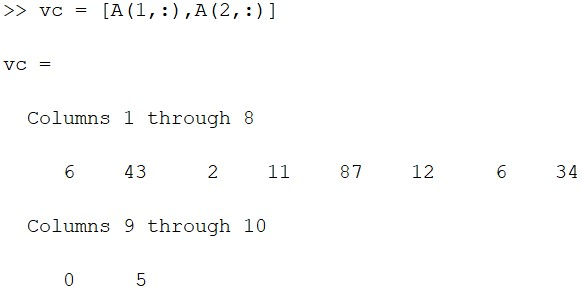
\includegraphics[width = 15cm]{img6c.jpg}
\end{figure}
\subsubsection{Crear un vector fila de seis elementos llamado vd, que contenga los elementos de la segunda y la quinta columna de A.}
\begin{figure}[H]
    \centering
    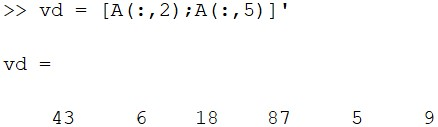
\includegraphics[width = 12cm]{img6d.jpg}
\end{figure}
\newpage
\subsection{Cree las siguientes matrices:}

\begin{equation*}
a =
\begin{pmatrix}
15 & 3 & 22 \\
3 & 8 & 5 \\
14 & 3 & 82
\end{pmatrix}
\end{equation*}

\begin{equation*}
b =
\begin{pmatrix}
1 \\
5 \\
6
\end{pmatrix}
\end{equation*}

\begin{equation*}
c =
\begin{pmatrix}
12 & 18 & 5 & 2
\end{pmatrix}
\end{equation*}

\begin{figure}[H]
    \centering
    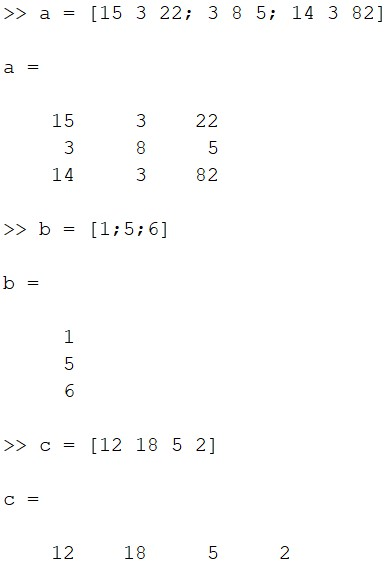
\includegraphics[width = 12cm]{img7.jpg}
\end{figure}
\newpage
Utilice las matrices a, b y c para:

\subsubsection{Cree una matriz llamada d a partir de la tercera columna de la matriz a.}
\begin{figure}[H]
    \centering
    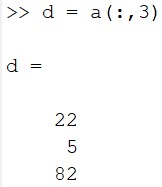
\includegraphics[width = 6cm]{img7a.jpg}
\end{figure}
\subsubsection{Combine la matriz b y la matriz d para crear la matriz e, una matriz bidimensional con tres filas y dos columnas.}
\begin{figure}[H]
    \centering
    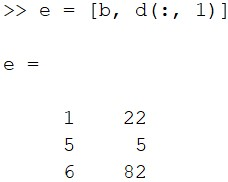
\includegraphics[width = 5cm]{img7b.jpg}
\end{figure}

\subsubsection{Combine la matriz b y la matriz d para crear la matriz f, una matriz unidimensional con seis filas y una columna.}
\begin{figure}[H]
    \centering
    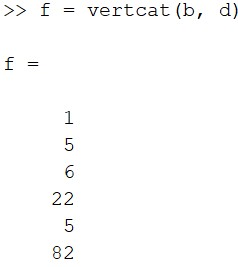
\includegraphics[width = 6cm]{img7c.jpg}
\end{figure}
\subsubsection{Cree una matriz g a partir de la matriz a y los primeros tres elementos de la matriz c, con cuatro filas y tres columnas.}
\begin{figure}[H]
    \centering
    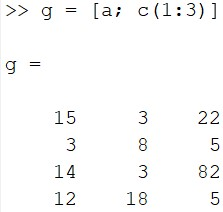
\includegraphics[width = 5cm]{img7d.jpg}
\end{figure}
\subsubsection{Cree una matriz h con el primer elemento igual a a1,3, el segundo elemento igual a c1,2 y el tercer elemento igual a b2,1.}
\begin{figure}[H]
    \centering
    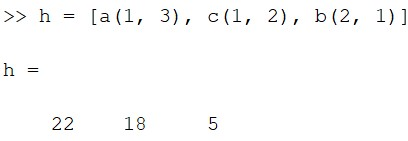
\includegraphics[width = 10cm]{img7e.jpg}
\end{figure}


\subsection{Cree la siguiente matriz:}

\begin{equation*}
\centering
A =
\begin{pmatrix}
1 & 2 & 3 & 4 & 5 & 6 & 7 \\
2 & 4 & 6 & 8 & 10 & 12 & 14 \\
21 & 18 & 15 & 12 & 9 & 6 & 3 \\
5 & 10 & 15 & 20 & 25 & 30 & 35
\end{pmatrix}
\end{equation*}

\begin{figure}[H]
    \centering
    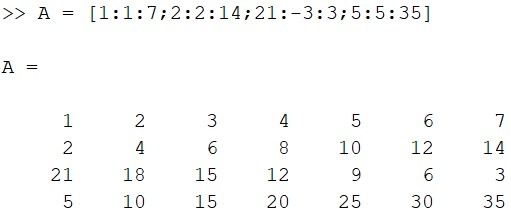
\includegraphics[width = 15cm]{img8.jpg}
\end{figure}

\subsubsection{Cree una matriz B de 3 × 4 a partir de la primera, tercera y cuarta fila, y de la primera, tercera, quinta y septima columna de la matriz A.}
\begin{figure}[H]
    \centering
    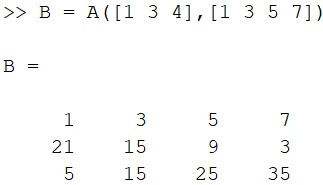
\includegraphics[width = 10cm]{img8a.jpg}
\end{figure}
\subsubsection{Cree un vector fila de 16 elementos llamado u, a partir de los elementos de la tercera fila y de la quinta a la septima columna de la matriz A.}
\begin{figure}[H]
    \centering
    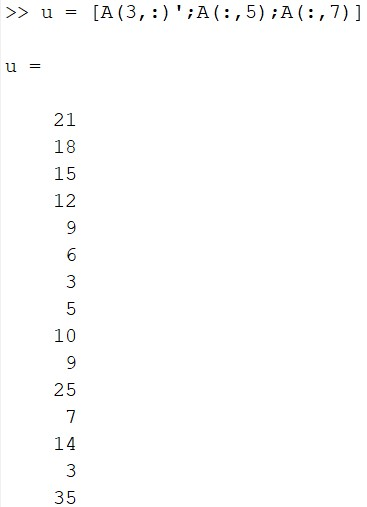
\includegraphics[width = 11cm]{img8b.jpg}
\end{figure}

\subsection{Cree una matriz de 5 × 7 en la cual la primer fila contenga los numeros: 1 2 3 4 5 6 7, la segunda fila contenga: 8 9 10 11 12 13 14, la tercera fila contenga los numeros del 15 al 21, y ası sucesivamente. A partir de esta matriz, cree otra nueva de 3 × 4 compuesta por las filas 3 a la 5 y las columnas de la 4 a la 7 de la primera matriz.}


\begin{figure}[H]
    \centering
    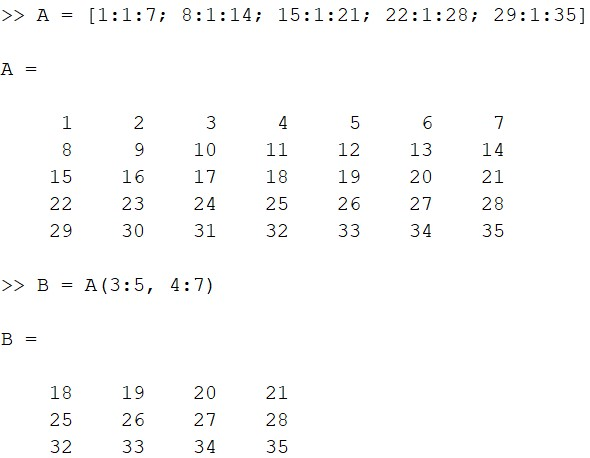
\includegraphics[width = 18cm]{img9.jpg}
\end{figure}

\
\
\

\section{Conclusion}

Esta practica, ademas de permitirnos practicar el uso de arreglos nos da una vision mas avanzada de los usos y formas de obtener estos.

\end{document}